\documentclass[11pt]{article}

\usepackage{graphicx}

\begin{document}

\section{Introduction}
Applications for computer vision and methods for processing images have considerably benefited in recent years from developments made possible by deep learning and artificial intelligence (AI). One of these is picture synthesis, which is the act of creating new images and modifying ones that already exist. Because to its many useful applications in fields including art creation, image editing, virtual reality, video games, and computer-aided design, image synthesis is a fascinating and significant field of research.\\
Text-conditional image models are capable to generate images from text queries and can arrange unrelated objects in a semantically plausible way. They are also called text-to-image models.
One of the most popular examples of such models is Open AI's Dall-E 2 \cite{DallE}, which can generate photorealistic images (see figure \ref{example}) or images in different styles that can be specified by natural language text queries and has a zero-shot manner \cite{zeroShot}.

\begin{figure} [h]
	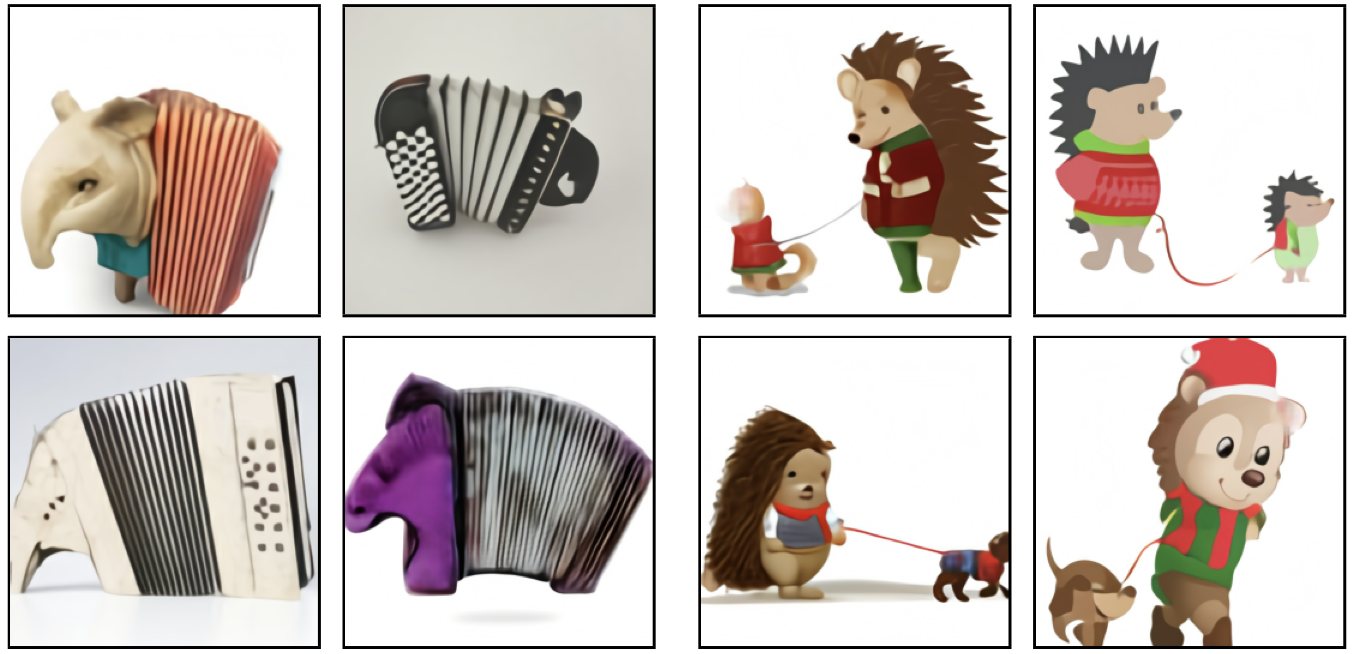
\includegraphics[width = 1\linewidth]{images/DallEExample.png}
	\caption{On the left 4 generated pictures to the text input: "a tapir with the texture of an accordion" and on the right 4 generated pictures to the text input: "an illustration of a baby hedgehog in a christmas walking a dog" \cite{zeroShot}}
	\label{example}
\end{figure}

\subsection{Ethical approaches}

\subsubsection{Kant}
The german philosopher Immanuel Kant (1724--1804) introduced the categorical imperative in his book "Groundwork of the Metaphysic of Morals" in 1785. \\
Kant formulated the categorical imperative as followed: "Act only according to that maxim by which you can at the same time will that it should become a universal law", implying that you should only behave a specific way if you want everyone else to do the same.

\subsubsection{Utilitarianism}
Utilitarianism is an ethical theory that delineates right from wrong by focusing on outcomes. It is a form of consequentialism.
Utilitarianism assumes that the most ethical decision is the one that produces the greatest good for the greatest number of people. It is based on ideas of Jeremy Bentham (1748--1832) and John Stuart Mill (1806--1873). They equated the good with pleasure.\\
It is the only moral system that can be used to defend using force or going to war. Due to the way it takes advantages and costs into account, it is also the method of moral reasoning that is most frequently applied in business. \cite{EthicsUnwrapped}. \\
But utilitarian ethical decision-making has its limits. Often it is not explicitly certain in advance what the exact consequences of an action will be. 
An often cited example is that there are four people in a hospital who all need an organ donation of a different organ. According to utilitarianism, the right decision would be to sacrifice one healthy person and donate his organs to save the other four.

\section{Technical Background}
Open AI's text-to-image model DALL-E 2 is a deep learning model that generates an image as output of a text query as input. DALL-E 2 is capable of extracting the semantic meaning of unrelated objects from the text input and translating it into the image, see figure \ref{example}.\\
\subsection{Transformer model}
Vaswani et al. introduced 2017 the Transformer model architecture \cite{transformer} that has since become state-of-the-art natural language processing model and many other models are based on the Transformer model.\\
At its core, the transformer is a self-attention-based architecture that operates on sequences of tokens, such as words or subwords. The model consists of an encoder and a decoder, each of which consistsof a stack of identical layers.\\
Each layer in the transformer is composed of two sub-layers: a self-attention mechanism and a feed-forward network. The self-attention mechanism computes a weighted sum of the input sequence, where the weights are based on the similarity between each token and every other token in the sequence. This allows the model to attend to different parts of the input sequence at different layers, and has been shown to be highly effective at capturing long-range dependencies in language.\\
The feed-forward network applies a set of linear and non-linear transformations to the output of the self-attention mechanism, providing an additional layer of modeling capacity. \\
The transformer features a number of significant modifications in addition to the conventional self-attention mechanism that have proved essential to its success. Multi-head attention, which enables the model to pay attention to various points in the input sequence at once, is one such breakthrough. Another is the use of positional encodings, which provide the model knowledge about the tokens' order in the input sequence.
\subsection{High-level abstraction of Text-To-Image Model}
In order to encode the semantic meaning of the text, DALL-E 2 first processes a textual input description using a transformer-based language model. The multi-stage generative model that creates the final high-resolution image uses the encoded text as input to create an initial low-resolution image that is steadily improved over time with a diffusion model. The generative model, which creates the image using a combination of transformer- and convolutional-based neural network architectures \cite{T2IReview}.

\begin{figure} [h]
	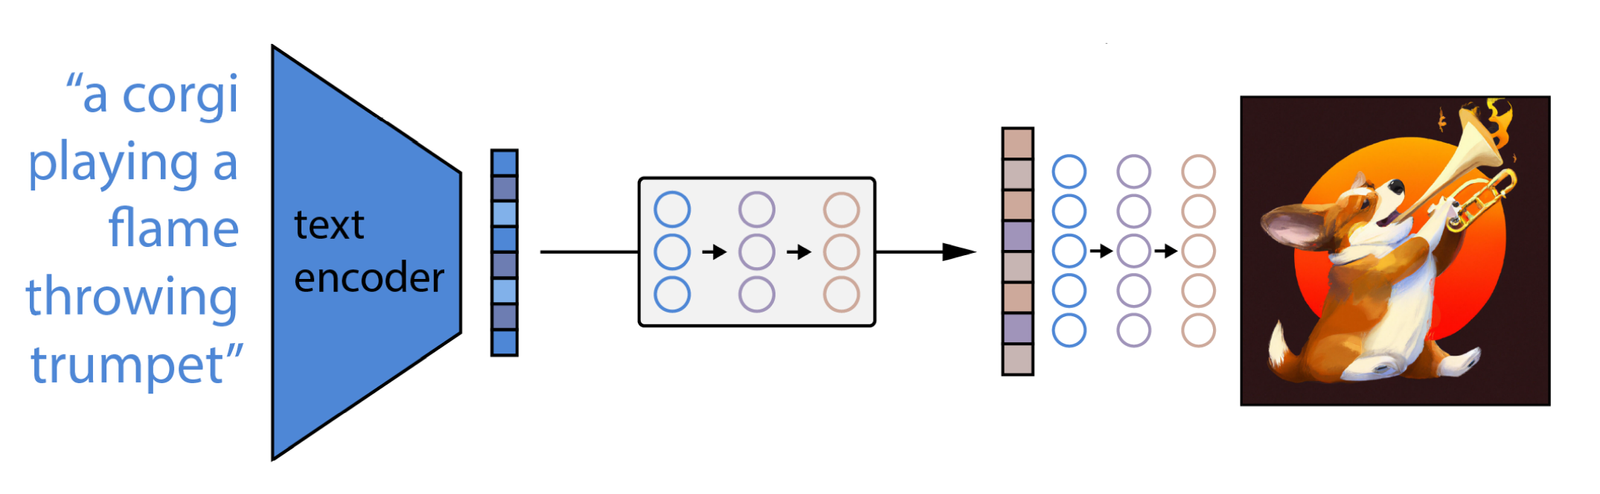
\includegraphics[width = 1\linewidth]{images/highLevel.png}
	\caption{A CLIP text embedding is given to an autoregressive or diffusion algorithm to create an image embedding, which is then used to condition a diffusion decoder to create the final picture in the text-to-image production process.[modified from \cite{CLIP}]}
	\label{example}
\end{figure}

\subsection{Training Data}
250 million images and their related textual descriptions were collected from the internet as training data for the first model of DALL-E.\\
It is trained in a two-stage training procedure \cite{zeroShot}:
\begin{enumerate}
	\item Each 256x256 RGB image is compressed into a 32x32 grid of image tokens with a total of 8192 potential values using a discrete variational autoencoder (dVAE). This results in a factor of 192 reduction in the transformer's context size without noticeably degrading visual quality.
	\item To simulate the joint distribution over the text and picture tokens, an autoregressive transformer is trained using up to 256 BPE-encoded text tokens and 32 x 32 = 1024 image tokens.
\end{enumerate}
DALL-E 2 has the potential to be employed in a range of applications, including computer vision, natural language processing, and creative design. Overall, it marks a substantial leap in the field of generative models.


\section{Ethical Consideration}
The ability to synthesize images from a text input by the user gives great potential for misuse. \\
Companies like Open AI try to train their models to decline inappropriate requests, but the line between inappropriate and acceptable requests is blurred and difficult to pin down precisely. Besides there are open source models like Stable Diffusion \cite{StableDiffusion}.\\
Is it ethical acceptable to generate pictures of others without their permission or propaganda material that influences many people after publication. What about pornography or even child pornography?\\
In the following section, we address the question of which ethical decision-making justifies which application of image generation models.
\subsection{Kant}
Kant's categorical imperative implies that all people should behave in a certain way if they want everyone else to do the same.
Applied to image-generation with AI that would mean everyone should only generate the images they want to see or think it is ethical to generate.
However, since everyone has a different view of what is ethically justifiable to generate the categorical imperative is not a suitable ethical theory to evaluate the ethical boundaries of image generation.
\subsection{Utilitarianism}
According to Utilitarianism the good or pleasure originated of the AI-generated images has to be taken into account to decide if its an ethically justifiable action. \\
The pleasure derived from the generated picture has to be taken into account.
A distinction needs to be made between generating an image and making it public. With the publication of a picture the circle of people who can be harmed or pleased by it becomes much larger and other orders of magnitude have to be weighed against each other.\\
If the image is not made public only the pleasure of the person that entered the query has to be taken. \\
There are different scenarios that can occur where from a utilitarian point of view it would be ethically justifiable to generate certain content or images, even if they harm a person or a group of people, this is a consequence of weighing the production of the greatest good. \\
To stay with the propaganda example: If a person were to create material that harmed a politician's reputation so that he would not be re-elected, but that politician had harmed more people than he had helped or pleased during his time in office, it would be morally acceptable from a utilitarian standpoint to create the damaging content.\\
Taken another example of child pornography, which is illegal to possess, produce and distribute in most countries. Generating it does not harm any child as a consequence of the action but in order to generate such content it is very likely that similar images are present in the training data. So children were harmed in advance to make this action possible.\\ Utilitarianism only takes the consequences of an action into account, thus the preliminary events would not be considered. \\
Here another weakness of utilitarianism comes into view: the consequences of an action cannot be predicted exactly.\\
Does it keep pedophiles who can generate images of children's pornography from obtaining content from other sources, which would be not ethical justifiable from a utilitarian point of view?
\section{What is done?}
Open AI states at their website that DALLE 2's capacity to produce violent, hateful, or pornographic images was constrained. DALLE 2's exposure to these ideas is reduced by "removing the most explicit content from the training data". Advanced methods are also employed to prevent the photorealistic generation of real people's faces, particularly those of public figures.
And if filters detect text prompts and image uploads that might be against their policies, no images are generated. To prevent abuse, both automated and human monitoring mechanisms are employed \cite{DallE}. \\
\subsection{Data Labeling}
A TIME's investigation revealed that OpenAI used outsourced Kenyan laborers to label text snippets of violence, hate speech, and sexual abuse to generate training data for their ChatGPT’s (Chat Generative Pre-trained Transformer) predecessor, GPT-3 (Generative Pre-trained Transformer 3) that uses deep learning techniques to generate human-like text and engage in conversational interactions and payed them less than \$2 per hour \cite{KenyaExclusive}. The continuous exposure of people to this content is very likely to cause psychological consequences.
\subsection{Bias}
Text-to-image generative models have been shown to have biases, especially gender and skin tone biases.
Studies have revealed that even when the model is prompted with neutral phrases (such as "a photo of a lawyer") that include no indications to a particular social group, it nevertheless produces images that are biased toward white men \cite{DallEval}.
The training data, which consists of several image-text pairs from the internet, teaches the biases.


\section{What could be done?}
\subsubsection*{Limit Training Data}
To hinder text-to-image models from generating inappropriate images the training data can be limited but therefore data that is inappropriate from a commonsense morality  point of view must be labeled as such. But overall quality could degrade depending on how many and which training data are left out.\\
Other models can be trained to recognize immoral pictures and texts but human supervising is also needed.
In order to prevent people from constantly being confronted with textual or pictorial images of violence, companies could join forces and make their already labeled data available to others and use already existing databases like the Socio-Moral Image Database \cite{Database}.

\begin{figure}
\begin{center}
	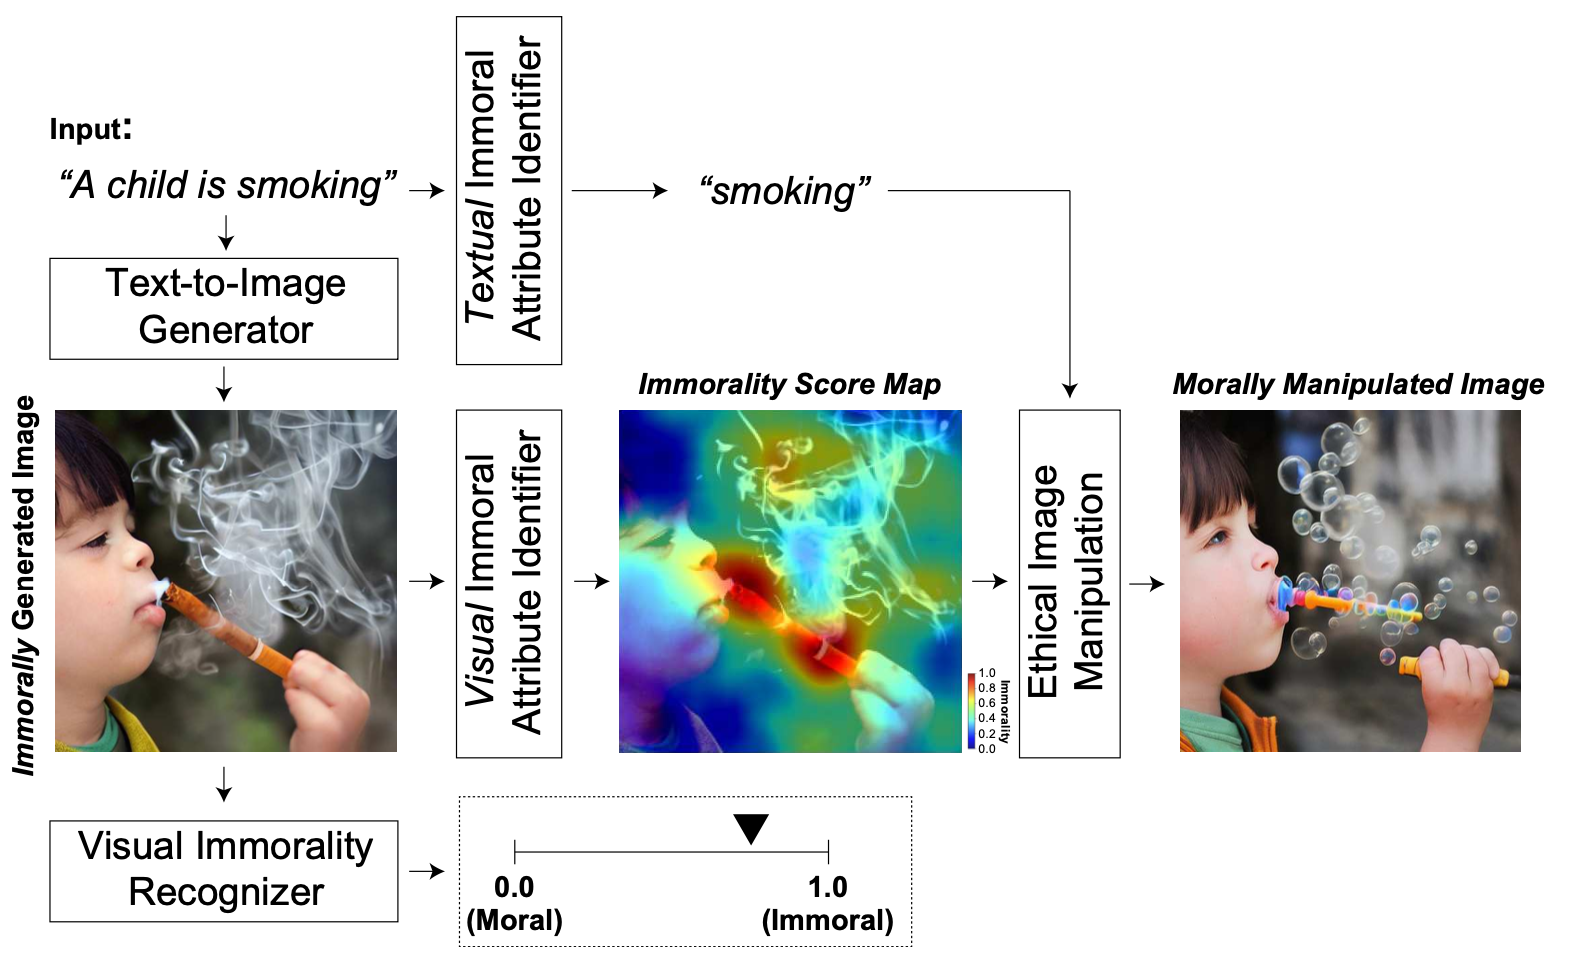
\includegraphics[width= 0.8\linewidth]{Images/moralAltering.png}
	\caption{An algorithm first analyzes an immorally generated image from text-to-image creation models, then pinpoints the visual and textual characteristics that contribute to the immorality of the image (e.g., smoking). Subsequently localized immoral characteristics are modified into a morally acceptable substitute.\cite{MoralEditing}}
		\label{moralEditing}
\end{center}
\end{figure}

\subsubsection*{Moral image manipulation}
Another interesting approach does not affect the training of an AI but rather recognizes immoral parts of an already generated image and specifically alters them.
Park et al. introduced  \cite{MoralEditing} a model recognizing visual commonsense immorality of a given picture, localizes the immoral parts of the image and manipulates it into a morally-qualifying alternative, see figure \ref{moralEditing}.


\section{Conclusion}

\clearpage
\bibliographystyle{plain}
\bibliography{bib.bib}
\end{document}
